%%%%%%%%%%%%%%%%%%%%%%%%%%%%%%%%%%%%%%%%%
% Short Sectioned Assignment
% LaTeX Template
% Version 1.0 (5/5/12)
%
% This template has been downloaded from:
% http://www.LaTeXTemplates.com
%
% Original author:
% Frits Wenneker (http://www.howtotex.com)
%
% License:
% CC BY-NC-SA 3.0 (http://creativecommons.org/licenses/by-nc-sa/3.0/)
%
%%%%%%%%%%%%%%%%%%%%%%%%%%%%%%%%%%%%%%%%%

%----------------------------------------------------------------------------------------
%	PACKAGES AND OTHER DOCUMENT CONFIGURATIONS
%----------------------------------------------------------------------------------------

\documentclass[paper=a4, fontsize=11pt]{scrartcl} % A4 paper and 11pt font size

\usepackage[T1]{fontenc} % Use 8-bit encoding that has 256 glyphs
%\usepackage{fourier} % Use the Adobe Utopia font for the document - comment this line to return to the LaTeX default
\usepackage[english]{babel} % English language/hyphenation
\usepackage{amsmath,amsfonts,amsthm,amssymb} % Math packages

\usepackage{sectsty} % Allows customizing section commands
%\allsectionsfont{\centering \normalfont\scshape} % Make all sections centered, the default font and small caps
\allsectionsfont{\centering}

\usepackage{fancyhdr} % Custom headers and footers
\pagestyle{fancyplain} % Makes all pages in the document conform to the custom headers and footers
\fancyhead{} % No page header - if you want one, create it in the same way as the footers below
\fancyfoot[L]{} % Empty left footer
\fancyfoot[C]{} % Empty center footer
\fancyfoot[R]{\thepage} % Page numbering for right footer
\renewcommand{\headrulewidth}{0pt} % Remove header underlines
\renewcommand{\footrulewidth}{0pt} % Remove footer underlines
\setlength{\headheight}{13.6pt} % Customize the height of the header

%\numberwithin{equation}{section} % Number equations within sections (i.e. 1.1, 1.2, 2.1, 2.2 instead of 1, 2, 3, 4)
%\numberwithin{figure}{section} % Number figures within sections (i.e. 1.1, 1.2, 2.1, 2.2 instead of 1, 2, 3, 4)
%\numberwithin{table}{section} % Number tables within sections (i.e. 1.1, 1.2, 2.1, 2.2 instead of 1, 2, 3, 4)

\setlength\parindent{0pt} % Removes all indentation from paragraphs - comment this line for an assignment with lots of text

\usepackage{caption}

\usepackage{algorithm}
\usepackage[noend]{algorithmic}

%\floatname{algorithm}{Procedure}
\renewcommand{\algorithmicrequire}{\textbf{Input:}}
\renewcommand{\algorithmicensure}{\textbf{Output:}}

\newtheorem{mydef}{Definition}
\theoremstyle{plain}
\newtheorem{lemma}{Lemma}


\usepackage{graphicx}
%\graphicspath{{//figures/}}

%\usepackage{epstopdf}
\usepackage[outdir=./]{epstopdf}

%----------------------------------------------------------------------------------------
%	TITLE SECTION
%----------------------------------------------------------------------------------------

\newcommand{\horrule}[1]{\rule{\linewidth}{#1}} % Create horizontal rule command with 1 argument of height

\title{	
\normalfont \normalsize 
\textsc{UPC - Discrete and algorithmic geometry} \\ [25pt] % Your university, school and/or department name(s)
\horrule{0.5pt} \\[0.4cm] % Thin top horizontal rule
\huge Problem sheet 2  \\ % The assignment title
\horrule{2pt} \\[0.5cm] % Thick bottom horizontal rule
}

\author{Simon Van den Eynde \\ Petar Hlad Colic} % Your name

\date{\normalsize\today} % Today's date or a custom date

\begin{document}

\maketitle % Print the title

\section{Matousek}
\subsection{2}
\subsubsection{Problem description}
We will use Lemma 5.1.2 (Duality preserves incidences) ii) in Matousek: 
Let $p$ be a point of $\mathbb{R}^{d}$ distinct from the origin and let $h$ be a hyperplane in $\mathbb{R}^d$ not containing the origin. Let $h^-$ stand for the closed half-space bounded by $h$ and containing the origin, while $h^+$ denotes the other closed half-space bounded by $h$. That is, if $h=\{x\in\mathbb{R}^d: \langle a,x\rangle=1\}$, then $h^-=\{x\in\mathbb{R}^d: \langle a,x\rangle\leq1\}$.
Then $p\in h^- \iff D_0(h)\in D_0(p)^-$.\\

Let us consider a pentagon which contains the origin. Let $v_i = D_0(l_i)$, where $l_i$ is the line containing the side $a_ia_{i+1}$. Then the points dual to the lines intersecting the pentagon $a_1a_2\ldots a_5$ fill exactly the exterior of the convex pentagon $P_{ex} = v_1v_2\ldots v_5$.

\subsection{solution}
So take a point $p$ outside $P_{ex}$. Because $P_{ex}$ is convex there exists an edge $v_iv_{i+1}$ (we assume here that $v_{5+1}=v_1$) with supporting line $h$, such that $p$ lies in the halfplane $h^+$ (not containing the origin). Because duality preserves incidences we find $D_0(h)\in D_0(p)^+$. Now since $D_0(h)=D_0(D_0(a_{i+1}))=a_{i+1}$, we find that the line segment $[0,a_{i+1}]\cap D_0(p)\neq \varnothing$. So $D_0(p)$ intersects $P_{ex}$.

Why is $v_iv_{i+1}=D_0(a_{i+1})$?
\begin{align*}
v_i&=D_0(a_{i}a_{i+1}),& v_j=D_0(a_{i+1}a_{i+2})\\
\implies &D_0(v_i)=a_ia_{i+1},& D_0(v_j)=a_{i+1}a_{i+2}\\
\implies &D_0(v_i)D_0(v_j)=a_{i+1}\\
\implies &D_0(a_{i+1})=v_iv_j
\end{align*}

Now analogous to the first part we can take a point $p$ inside $P_{ex}$ then we find $v_{i}v_{i+1}$ with a supporting line $h$ such that $p\in h^-$. We find $D_0(h)=a_{i+1}\in D_0(p)^-$ So that $D_0(p)$ intersects the line $a_{i+1}$ outside the pentagon. Because $D_0(p)$ is perpendicular to $a_{i+1}$ it will never intersect the convex polygon

\subsection{3}
\begin{align*}
X^{*} &= \{y\in \mathbb{R}^{d} : \langle x,y\rangle \leq 1, \forall x \in X\}\\
X^{**} &= \{y\in \mathbb{R}^{d} : \langle x,y\rangle \leq 1, \forall x \in X^{*}\}
\end{align*}
 
Now because $\forall x\in X,\forall y \in X^{*} : \langle x,y\rangle \leq 1 \implies x\in X^{**}$. Also clearly $0\in X^{**}$. Since $X^{**}$ closed and convex we find $conv(X\cup 0)\subset X^{**}$.

The separation theorem says that for a closed set $Z$: $conv(Z)=\bigcap$(all closed halfspaces that contain Z).
So $conv(X\cup 0)$ is the intersection of all closed halfspace that contain $0$ and $X$.

\section{$C_4(7)$}
\subsection{(a)}
We will first calculate the $f$-vector of $C_4(7)$.
\begin{itemize}
\item $f_0=7$
\item $f_1= \binom{7}{2} = 21$, because $C_4(7)$ is neighborly
\item $f_3 = 14$, we counted this in class, using Gale's evenness criterium.
\end{itemize}

Define $h_k = \sum_{i\geq k}^{d} f_{i}(-1)^{(i-k)}\binom{k}{i} $, with $f_{-1}=f_{d}=1$. Then the Dehn-Sommerville equations learn us that $h_i=h_{d-i}$.\\
We find $h_0=f_0-f_1+f_2-f_3+f_4=7-21+f_2-14+1=f_2-27$ and $h_4=f_4=1$. Now $h_0=h_4\implies f_3=28$.

So $f(C_4(7))=(7,21,28,14)$. And we find $f(C_4(7)^\Delta)=(14,28,21,7)$
\section{$24$-cell}

$$ P = conv\left\lbrace \pm e_i \pm e_j : 1\leq i,j\leq 4,\, i\neq j \right\rbrace$$

\textbf{Notation}: we'll note all vertices as pairs $(i,j)$ such that $ -4 \leq i,j \leq 4$ and $i \neq 0 \neq j$ and $i \neq j$. Note that $(i,j)=(j,i)$ as $e_i+e_j = e_j + e_i$.

\textbf{0-dimmensional faces (vertices):} All $4 \cdot {4 \choose 2} = 24$ vertices $(i,j)$

\textbf{1-dimmensional faces (edges):} Two vertices are adjacent if they share exactly one common vector from the basis. That is:
$$(i,j) \sim (k,l) \iff (i=k,\vert j \vert \neq \vert l \vert) \vee (i=l,\vert j \vert \neq \vert k \vert) \vee (j=k,\vert i \vert \neq \vert l \vert) \vee (j=l,\vert i \vert \neq \vert k \vert)$$
Nottice that $(i,j)$ and $(i,-j)$ as the segment $(i,j)(i,-j)$ has length 2 unlike the edges that have length $\sqrt{2}$.

So, each vertex has 8 adjacent vertices. As every edge is double counted, the total number of edges is $\frac{24 \cdot 8}{2} = 96$.

\textbf{2-dimmensional faces (faces):} choose any 3 $a_1,a_2,a_3$ such that $a_1 \sim a_2, a_2 \sim a_3, a_1 \nsim a_3$.
So if $a_1 = (i,j)$ with $\vert i \vert \neq \vert j \vert$, then $a_2 = (j,k)$ with $\vert i \vert \neq \vert k \vert \neq \vert j \vert$ and $a_3 = (k,l)$ with $\vert l \vert \neq \vert i \vert, \vert j \vert, \vert k \vert$. The vertex $a_4=(l,j)$ and $a_5=(i,k)$ are adjacent to $a_1,a_2,a_3$. This proves that for any two adjacent edges, either they are in the same triangle, or they are in two adjacent triangles. So all faces are triangles.

Every pair of adjacent vertices has 4 vertices that are adjacent to both. As all faces are triangles and every triangle is counted 4 times for each edge, the total number of triangles is $\frac{96 \cdot 4}{4} = 96$ 

\textbf{3-dimmensional faces (cells):} choose any face $a_1,a_2,a_3$.

Then $a_1 = (i,j), a_2=(j,l), a_3=(l,i)$ for some $i,j,l$ such that $1 \leq \vert i \vert, \vert j \vert, \vert l \vert \leq 4$ and $\vert i \vert \neq \vert l \vert \neq \vert j \vert \neq \vert i \vert$. Choose $ 1 \leq \vert k \vert \leq 4 $ such that $\vert k \vert \neq \vert i \vert, \vert j \vert, \vert l \vert$ (there are only two possibilities: $k$ and $-k$). Consider the vertices $(j,k)$, $(i,k)$ and $(l,k)$. As we can see in Figure 1, the graph of this set of points is 4-regular, where all faces are triangles, there are 8 faces, and each vertex is incident to 4 faces. It is the graph of a regular octahedron.

So, all cells are regular octahedrons.

\begin{figure}[!htb]
\centering
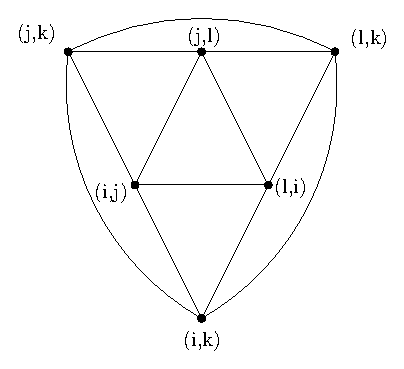
\includegraphics[scale=0.8]{figures/facet.eps}
\caption{24cell facet}
\label{fig:face}
\end{figure}

Given a vertex $(i,j)$, there are 4 possible pairs $\vert k \vert \neq \vert l \vert$ such that $\vert k \vert, \vert l \vert \neq \vert i \vert, \vert j \vert$ and that $(i,j),(i,k),(i,l),(j,k),(j,l),(k,l)$ form an octahedron. So every vertex is in 4 octahedrons. As all cells are counted 4 times, the total number of cells is $\frac{24 \cdot 4}{4} = 24$ \\

\underline{Face lattice} \\

A vertex $(i,j)$ is an endpoint of an edge $(i',j')(j',k')$ if and only if $\{i,j\} \subset \{i',j',k'\}$ \\

An edge $(i,j)(j,k)$ is an edge of a face $(i',j')(j',k')(k',i')$ if and only if either $j \in \{i',j',k'\}$ or $\{i,k\} \subset \{i',j',k'\}$ \\

A face $(i,j)(j,k)(k,i)$ is a face of a cell formed by $\{(i',j'),(i',k'),(i',l'),(j',k'),(j',l'),(k',l')\}$ if and only if $\{i,j,k\} \subset \{i',j',k',l'\}$.\\

\underline{Self-polar-duality} \\

We'll now flip the notation. Now, the vertices are noted as $\{i,j,k,l\}$. As seen in the face lattice (two cells share a face if the indices of the face are contained in the indices of both cells at the same time) two vertices $\{i,j,k,l\},\{i',j',k',l'\}$ are adjacent if and only if they share three indices. 

\end{document}
